% You can choose whether you prefer a single or double column appendix.
% Whatever you choose, you will need to stick to it throughout the appendix.
% For double column style, comment the next line.
\onecolumn

\appendix
\begin{appendices}

\section{Hochstenbach and Van Gent's findings on gentrification in Amsterdam neighborhoods}
\label{sec:apx:Hochstenbach}

    {\setlength{\intextsep}{0pt}
    \begin{figure}[h!]
        \centering
        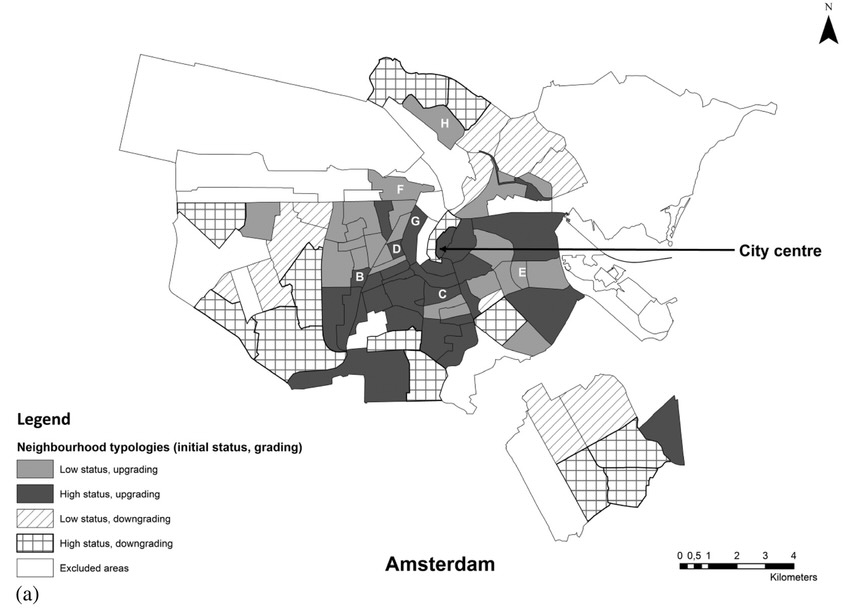
\includegraphics[width=0.8\textwidth]{media/methodology/neighbourhood-grading.jpg}
        \caption{Neighborhood initial status and grading \cite{hochstenbach_anatomy_2015}. Neighborhood initial status was defined as above- (high status) or below-average (low status) median income in 2004. Neighborhood grading was defined as an increase (upgrading) or decrease (downgrading) in the median income (corrected for inflation) during the period 2004–11. Note how Zuidoost and Nieuw-West were found to be downgrading, and Oud-West and Centrum-West - particularly De Jordaan - were found to be upgrading.}
        % \label{fig:SS_ins_sz}
    \end{figure}
    
    \begin{figure}[h!]
        \centering
        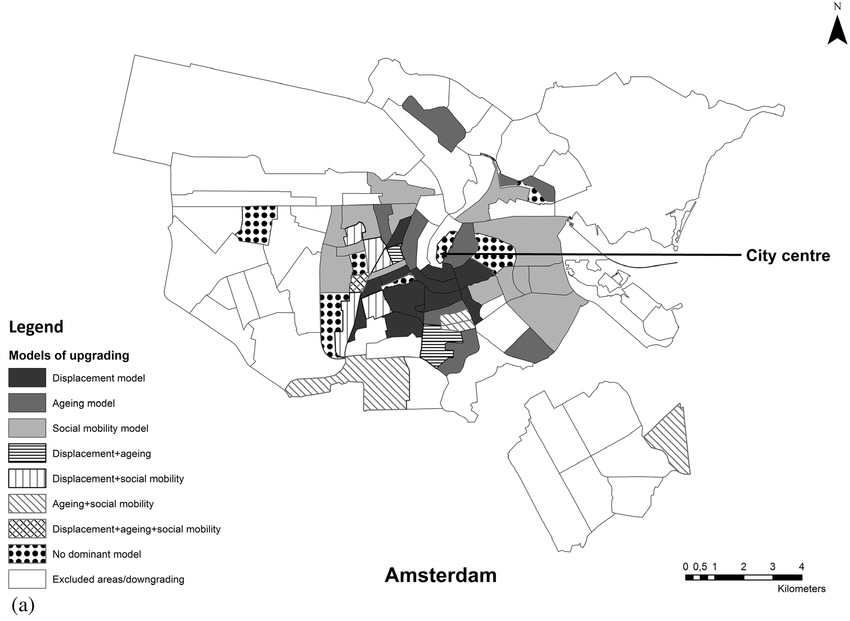
\includegraphics[width=0.8\textwidth]{media/methodology/neighbourhood_models.jpg}
        \caption{Neighborhood upgrades \cite{hochstenbach_anatomy_2015}. Displacement was defined as an above-average share of migration among low-income residents and an above-average share of migration among middle- or high-income residents. Social mobility was defined as an above-average share of low-income residents experiencing upward social mobility (and become middle- or high-income) while staying in the same neighbourhood. Ageing was defined as an above-average share of low-income residents ageing out of the core population. Note how Oud-West and Centrum-West - particularly De Jordaan - were found to have undergone social mobility, displacement, and ageing; while no such trend was found for Zuidoost and Nieuw-West.}
        % \label{fig:pano_ins_sz}
    \end{figure}
    }

\section{Extended data example images.}
\label{sec:apx:pano_example}

    \begin{figure}[H]
        \centering
        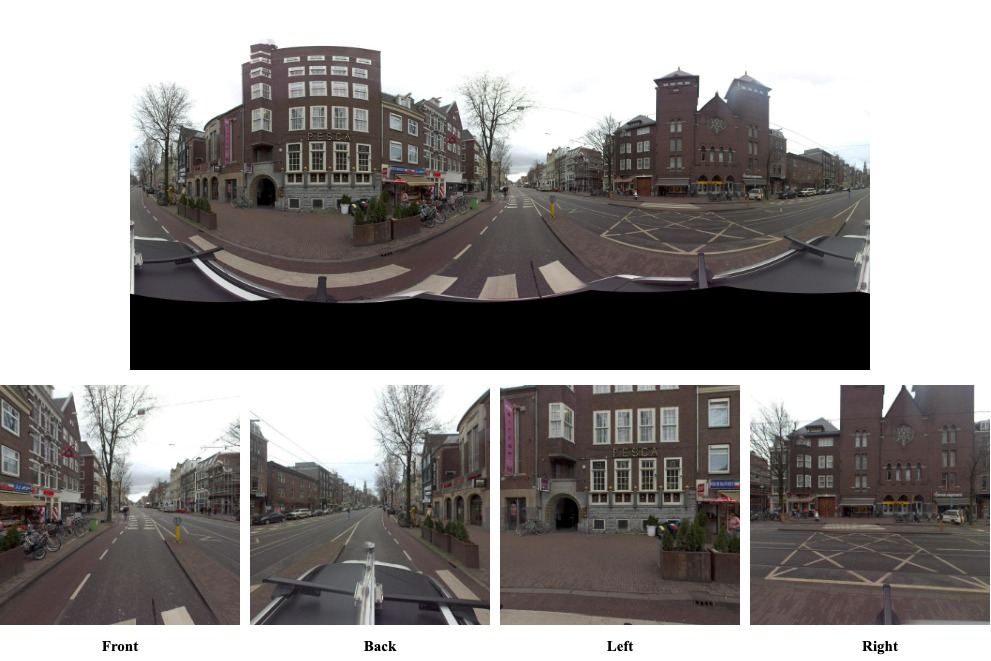
\includegraphics[width=0.8\textwidth]{media/methodology/data_ex/extended/pano_example.jpg}
        \caption{Example of the extended data.}
        % \label{fig:pano_example}
    \end{figure}


\section{Text instances size and aspect ratio.}
\label{sec:apx:instances}

    \begin{figure}[H]
        \centering
        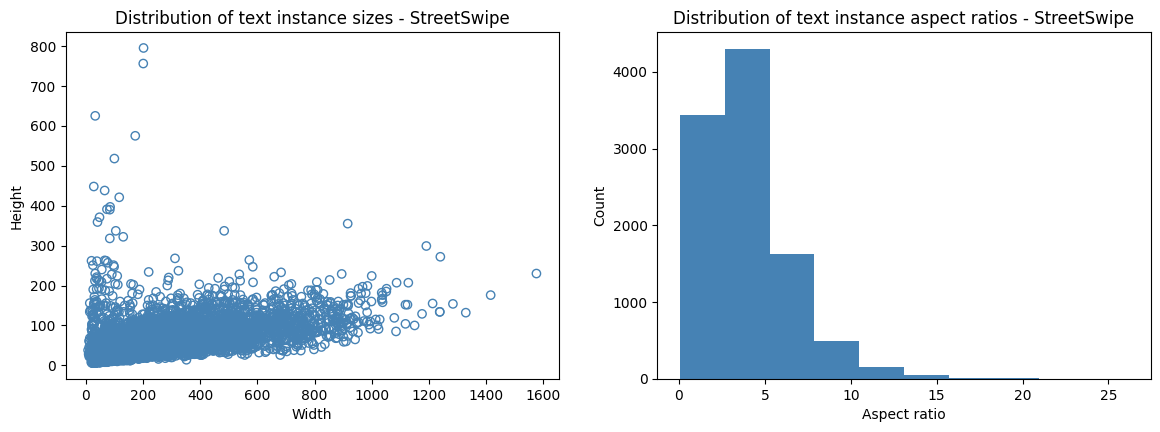
\includegraphics[width=\textwidth]{media/methodology/SS_ins_sz.png}
        \caption{StreetSwipe text instance size and aspect ratio}
        \label{fig:SS_ins_sz}
    \end{figure}
    
    \begin{figure}[H]
        \centering
        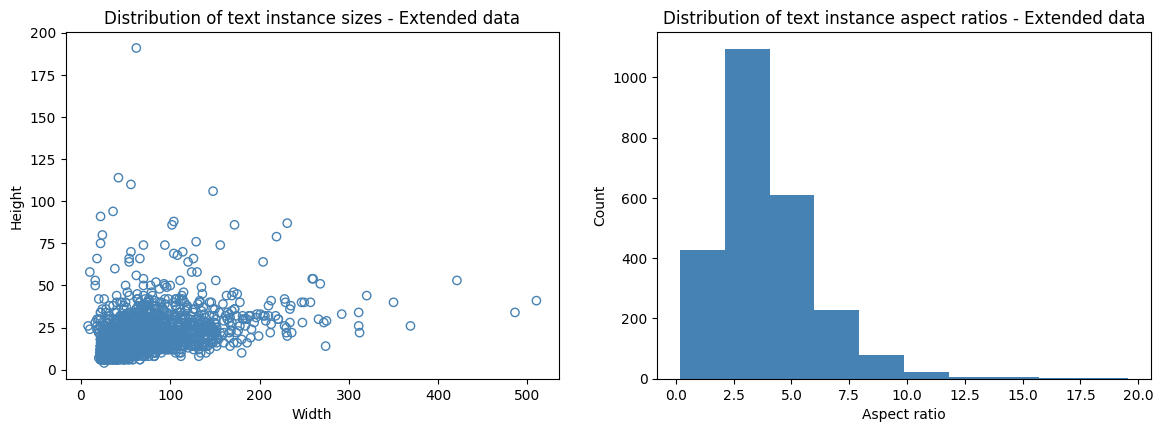
\includegraphics[width=\textwidth]{media/methodology/pano_ins_sz.png}
        \caption{Extended data text instance size and aspect ratio}
        \label{fig:pano_ins_sz}
    \end{figure}


\end{appendices}



